\begin{activity}{Oceanic vs. Continental Crust}

\section*{Purpose}

This activity applies the principle of isostatic equilibrium to oceanic and continental lithosphere. By comparing increasingly realistic column models, you will investigate why simple crust-only models fail and explore the role of lithospheric mantle structure and composition in supporting long-wavelength topography.

\section*{Learning Outcomes}

By the end of this activity, you should be able to:
\begin{itemize}
  \item Set up and solve isostatic balance equations for two-layer lithosphere columns.
  \item Explain the limitations of applying simple Airy-style reasoning to ocean--continent structure.
  \item Describe how mantle lithosphere composition (particularly garnet fraction) contributes to the density contrast between oceanic and continental mantle.
  \item Discuss the relationship between lithosphere composition, density, and long-term isostatic stability.
\end{itemize}

\subsection*{Theory: The General Isostatic Balance}

Isostatic equilibrium requires that pressure be equal at a common \emph{depth of compensation} beneath any two neighboring columns, regardless of how the mass within each column is distributed between layers. If a column is built from $N$ layers of thickness $h_i$ and density $\rho_i$, the pressure it exerts at its base is
\[
    P = g \sum_{i=1}^{N} \rho_i h_i .
\]
Because $g$ is common to every column, isostatic equilibrium between two columns reduces to equality of their layer-integrated mass per unit area:
\[
    \sum_{i=1}^{N} \rho_{i} h_{i} \Big|_{\text{Column 1}}
    \;=\;
    \sum_{i=1}^{N} \rho_{i} h_{i} \Big|_{\text{Column 2}} .
\]

\paragraph{Handling unequal column heights.} Real columns rarely have the same total height --- one may stand higher (positive elevation) or lower (e.g.\ beneath an ocean) than the other. To compare them at a common depth, extend the \emph{shorter} column downward with additional material of mantle density $\rho_m$ until both columns reach the same base level, the depth of compensation (Figure~\ref{fig:general_balance}). This filler thickness is not a separate physical layer --- it is simply the bookkeeping needed to align two columns of different height at a common depth. Written this way, elevation is not a separate term added to the balance; it is already accounted for as part of one column's total thickness.

\emph{Note:} If you are not sure in advance which column is higher, it does not matter which one you assign the elevation to --- assign it either way and solve. Placing it on the correct column gives a positive elevation; placing it on the other column simply gives the same result with a negative sign.

\begin{figure}[h]
\centering
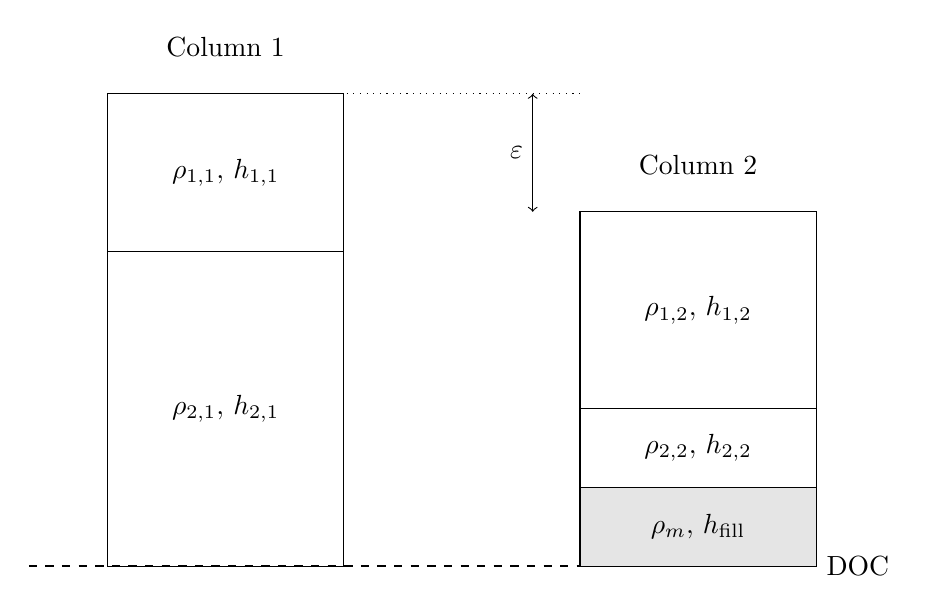
\begin{tikzpicture}[x=1cm,y=1cm]
   
    \def\baseA{0}      
    \def\baseB{-1.5}   
    \def\compdepth{-6} 
   
    % depth of compensation
    \draw[dashed, thick] (-1,\compdepth) -- (9,\compdepth)
        node[right] {DOC};
   
    % right column
    \draw (0,\baseA) rectangle node{$\rho_{1,1},\,h_{1,1}$} (3,\baseA-2);
    \draw (0,\baseA-2) rectangle node{$\rho_{2,1},\,h_{2,1}$} (3,\compdepth);
   
    % elevation label
    \draw[<->] (5.4,\baseA) -- (5.4,\baseB)
        node[midway,left] {$\varepsilon$};

   
    % left column
    \draw (6,\baseB) rectangle node{$\rho_{1,2},\,h_{1,2}$} (9,\baseB-2.5);
    \draw (6,\baseB-2.5) rectangle node{$\rho_{2,2},\,h_{2,2}$} (9,-5);
   
    % mantle column (on left)
    \draw[fill=gray!20] (6,-5) rectangle
        node{$\rho_m,\,h_{\mathrm{fill}}$} (9,\compdepth);

    \draw[dotted] (0,\baseA) -- (6,\baseA);

    \node at (1.5,\baseA+0.6) {Column 1};
    \node at (7.5,\baseB+0.6) {Column 2};
\end{tikzpicture}
\caption{Two generic lithospheric columns of different total height, aligned at a common depth of compensation (DOC). Column 2 stands lower by elevation $\varepsilon$; this is accounted for by an additional mantle-density filler thickness $h_{\mathrm{fill}}$ at its base, \emph{not} by adding a separate $\varepsilon$ term to the pressure balance.}
\label{fig:general_balance}
\end{figure}

\paragraph{What you will do in Part A.} You are given the layer thicknesses and densities for a continental and an oceanic column. One unknown density is missing. Write the pressure balance above for these two specific columns, extend the shorter column to the depth of compensation using mantle density, and solve for the missing density directly.

\section*{Part 1: Testing a Crust-only Isostasy Model}

\textbf{Given:}
\begin{multicols}{2}
\begin{description}[itemsep=0.0em, topsep=0.5em]
    \item [oceanic crust thickness:] $h_{oc} = \SI{7}{km}$
    \item [ocean depth:] $h_w = \SI{3.7}{km}$
    \item [seawater density:] $\rho_w = \SI{1030}{\du}$
    \item [continental crust thickness:] $h_{cc} = \SI{40}{km}$
    \item [continental crust density:] $\rho_{cc} = \SI{2850}{\du}$
    \item [continental elevation:] $\varepsilon = \SI{0.8}{km}$
    \item [mantle density:] $\rho_a = \SI{3330}{\du}$
\end{description}
\end{multicols}

\textbf{Instructions:}  
Assume isostatic compensation occurs solely through crustal thickness. Compute the density of the oceanic crust, $\rho_{oc}$, that balances the oceanic and continental columns. Compare your result with typical oceanic crust densities (\(\sim\)2900--\SI{3000}{\du}) and discuss why the crust-only assumption may fail.

\begin{figure}[h!]
    \centering
    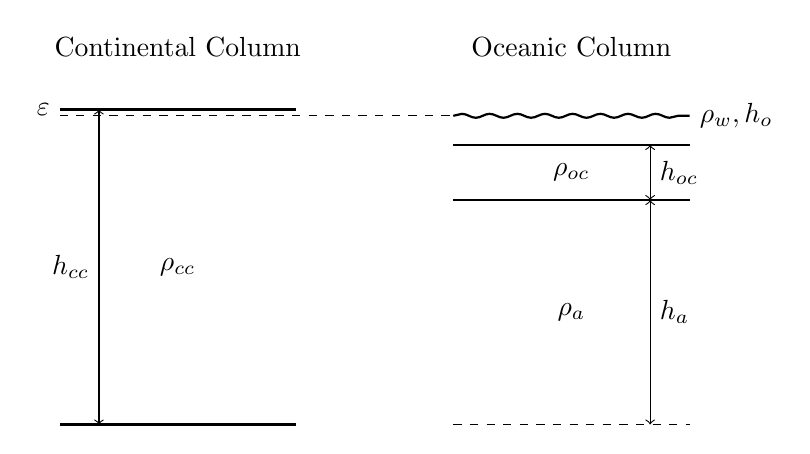
\begin{tikzpicture}[scale=0.1]

    \def\hcc{40}
    \def\elev{0.8}
    \def\hoc{7}
    \def\hw{3.7}

    % --- Continental column ---
    % Continental crust top (elevation h_c)
    \draw[thick] (0,\hcc) -- (30,\hcc);
    % Continental crust base
    \draw[thick] (0,0) -- (30,0);

    \node[left] at (0,\hcc) {$\varepsilon$};
    \draw[dashed] (0,\hcc-\elev) -- (50,\hcc-\elev);

    % --- Oceanic column ---
    % Mantle root below ocean (Airy root)
    \draw[dashed] (50,0) -- (80,0);
    % Oceanic crust base
    \draw[thick] (50,\hcc-\elev-\hw-\hoc) -- (80,\hcc-\elev-\hw-\hoc);
    % Oceanic crust top
    \draw[thick] (50,\hcc-\elev-\hw) -- (80,\hcc-\elev-\hw);
    % Water surface above ocean
    \draw[thick, decorate, decoration={snake, amplitude=0.25mm}] 
    (50,\hcc-\elev) -- (80,\hcc-\elev) node[right]{$\rho_w, h_o$};

    % --- Labels ---
    \node at (15,1.2*\hcc) {Continental Column};
    \node at (65,1.2*\hcc) {Oceanic Column};

    % --- Thickness arrows ---
    \draw[<->] (5,0) -- (5,\hcc) node[midway,left]{$h_{cc}$};
    \draw[<->] (75,\hcc-\elev-\hw) -- (75,\hcc-\elev-\hw-\hoc) node[midway,right]{$h_{oc}$};
    \draw[<->] (75,\hcc-\elev-\hw-\hoc) -- (75,0) node[midway,right]{$h_a$};

    % --- Density labels ---
    \node at (15,20) {$\rho_{cc}$};
    \node at (65,\hcc-\elev-\hw-\hoc/2) {$\rho_{oc}$};
    \node at (65,\hcc/2-\elev/2-\hw/2-\hoc/2) {$\rho_a$};

    \end{tikzpicture}
    \caption{Comparision of isostatic columns for the continental and oceanic crust for Part 1.}
    \label{fig:part1}
\end{figure}

\begin{questions}
    \question{One-layered isostasy.}
    Compute the required oceanic crust density $\rho_{oc}$.
    \answerbox[8cm]

    \question{Reflection.}
    Compare with expected oceanic crust densities and discuss why the simple crust-only model may not yield realistic values.
    \answerbox[3cm]
\end{questions}

\section*{Part 2: Two-layer Lithosphere Model}

\textbf{Given additional information:}
\begin{description}[topsep=0.5em,itemsep=0.0em]
    \item [Oceanic lithospheric mantle thickness] $h_{om} = \SI{75}{km}$
    \item [Oceanic lithospheric mantle density:] $\rho_{om} = \SI{3330}{\du}$
    \item [Continental lithospheric mantle thickness:] $h_{cm} = \SI{150}{km}$
    \item [Continental lithospheric mantle density:] $\rho_{cm} =\ ?$
    \item [Asthenosphere density:] $\rho_a = \SI{3320}{\du}$
\end{description}

\textbf{Instructions:}  
Let's add a two-layered lithosphere using average lithospheric thicknesses for the oceanic and continental settings.  Our goal will be to see what we can learn about the relative density difference between continental and oceanic mantle lithosphere.  In the process, we'll show how including the mantle lithosphere resolves the unrealistic crust-only result.

\begin{figure}[h!]
    \centering
    \begin{tikzpicture}[scale=0.1]

    \def\hcc{40}
    \def\elev{0.8}
    \def\hoc{7}
    \def\hw{3.7}
    \def\hcm{-40}
    \def\hom{-20}

    % --- Continental column ---
    % Continental crust top (elevation h_c)
    \draw[thick] (0,\hcc) -- (30,\hcc);
    % Continental crust base
    \draw[thick] (0,0) -- (30,0);
    % Continental lithosphere
    \draw[thick] (0,\hcm) -- (30,\hcm);

    \node[left] at (0,\hcc) {$\varepsilon$};
    \draw[dashed] (0,\hcc-\elev) -- (50,\hcc-\elev);

    % --- Oceanic column ---
    % Oceanic crust base
    \draw[thick] (50,\hcc-\elev-\hw-\hoc) -- (80,\hcc-\elev-\hw-\hoc);
    % Oceanic crust top
    \draw[thick] (50,\hcc-\elev-\hw) -- (80,\hcc-\elev-\hw);
    % Water surface above ocean
    \draw[thick, decorate, decoration={snake, amplitude=0.25mm}] 
    (50,\hcc-\elev) -- (80,\hcc-\elev) node[right]{$\rho_w, h_o$};
    % Mantle lithosphere
    \draw[thick] (50,\hom) -- (80,\hom);
    % Mantle root below ocean (Airy root)
    \draw[dashed] (50,\hcm) -- (80,\hcm);

    % --- Labels ---
    \node at (15,1.2*\hcc) {Continental Column};
    \node at (65,1.2*\hcc) {Oceanic Column};

    % --- Thickness arrows ---
    \draw[<->] (5,0) -- (5,\hcc) node[midway,left]{$h_{cc}$};
    \draw[<->] (5,0) -- (5,\hcm) node[midway,left]{$h_{cm}$};

    \draw[<->] (75,\hcc-\elev-\hw) -- (75,\hcc-\elev-\hw-\hoc) node[midway,right]{$h_{oc}$};
    \draw[<->] (75,\hcc-\elev-\hw-\hoc) -- (75,\hom) node[midway,right]{$h_{om}$};
    \draw[<->] (75,\hom) -- (75,\hcm) node[midway,right]{$h_a$};

    % --- Density labels ---
    \node at (15,20) {$\rho_{cc}$};
    \node at (15,\hcm/2) {$\rho_{cm}$};
    \node at (65,\hcc-\elev-\hw-\hoc/2) {$\rho_{oc}$};
    \node at (65,\hom+\hcc/2-\elev/2-\hw/2-\hoc/2-\hom/2) {$\rho_{om}$};
    \node at (65,\hom+\hcm/2-\hom/2) {$\rho_a$};

    \end{tikzpicture}
    \caption{Comparision of isostatic columns for the continental and oceanic crust for Part 2.}
    \label{fig:part2}
\end{figure}

\begin{table}[h!]
    \centering
    \caption{Modal proportions of minerals in the oceanic and continental lithospheres.}
    \label{tab:modes}
    \begin{tabular}{lcc}
        \toprule
        \textbf{Mineral} &
        \textbf{Oceanic} &
        \textbf{Continental} \\
        \midrule
        olivine & 75 & 60 \\
        orthopyroxene & 25 & 17 \\
        clinopyroxene & 10 & 11 \\
        garnet & 0 & 12 \\
        \bottomrule
    \end{tabular}
\end{table}
\FloatBarrier

Oceanic lithospheric mantle is assumed to be composed of depleted peridotite with a density of \(\rho_{om} = \SI{3330}{\du}\). Continental lithospheric mantle may contain a higher proportion of garnet.

\begin{description}[itemsep=0.0em, topsep=0.5em]
    \item [Density of depleted mantle (peridotite):] \(\rho_d = \SI{3330}{\du}\)
    \item [Density of garnet:] \(\rho_g = \SI{3600}{\du}\)
\end{description}

\begin{questions}[resume]
    \question{Two-layered isostasy.}
    Setup the isostatic equations for a two-layered mantle lithosphere.  If we assume an average oceanic crustal density $\rho_{oc} = $2900--\SI{3000}{\du}, what density of the continental mantle lithopshere?
    \answerbox[8cm]

    \question{Explain.}
    Explain how including the mantle lithosphere resolves the unrealistic density obtained in the crust-only case.
    \answerbox[4cm]

    \question{Discuss.}
    Discuss the role of garnet fraction in the continental lithospheric mantle for the density contrast. Compute the percentage difference garnet between the oceanic and continental lithsophere and compare your result with the modal proportions in Table~\ref{tab:modes}.
    \answerbox[5cm]
\end{questions}

\section*{Key Ideas}

\textbf{An unrealistic parameter value is diagnostic, not just wrong.} When solving a balance forces a physical property outside its plausible range (as with the required oceanic crust density here), that is a signal about what the model is missing, not merely an error to note and move past. The next step is always to ask what layer, mechanism, or assumption was left out.

\textbf{Density contrast, not absolute density, drives isostatic balance.} What matters in every column comparison is the difference between adjacent layers' densities, not their individual values. This is why even modest compositional differences between two otherwise similar layers can carry real isostatic consequences.

\textbf{Buoyancy depends on composition as much as thickness.} A thick layer is not automatically a heavy one --- its contribution to the balance depends on what it is made of. Any two properties that trade off in a balance (here, thickness and density) mean you cannot interpret one without also considering the other.

\textbf{Adding a layer resolves one unknown but introduces others.} Moving from a crust-only to a two-layer model produced a more realistic result, but only by introducing a new density that itself had to be constrained.  Extending a model to fix an implausible result is rarely free --- it is a trade of one assumption for another, better-motivated one.

\end{activity}